\documentclass[aspectratio=169]{beamer}
\usepackage{fontspec}
\usepackage{polyglossia}
\usepackage{color}
\usepackage{listings}
\setdefaultlanguage{russian}
\usepackage{csquotes}
\usetheme{metropolis}
\metroset{background=light}
\metroset{sectionpage=none}
\metroset{numbering=fraction}

\definecolor{ssaublue}{RGB}{77,144,205}
\setbeamercolor{frametitle}{fg=white, bg=ssaublue}
\setbeamercolor{title separator}{fg=ssaublue}

\setmainfont[
    Path = ../fonts/elektratextpro/,
    Extension = .otf,
    UprightFont = elektratextpro,
    BoldFont = elektratextpro_bold,
    ItalicFont = elektratextpro_italic,
    BoldItalicFont = elektratextpro_bolditalic
]{elektratextpro}

\setsansfont[
    Path = ../fonts/elektratextpro/,
    Extension = .otf,
    UprightFont = elektratextpro,
    BoldFont = elektratextpro_bold,
    ItalicFont = elektratextpro_italic,
    BoldItalicFont = elektratextpro_bolditalic
]{elektratextpro}

\setmonofont[
    Path = ../fonts/elektratextpro/,
    Extension = .otf,
    UprightFont = elektratextpro,
    BoldFont = elektratextpro_bold,
    ItalicFont = elektratextpro_italic,
    BoldItalicFont = elektratextpro_bolditalic
]{elektratextpro}

\newfontfamily\cyrillicfont[
    Path = ../fonts/elektratextpro/,
    Extension = .otf,
    UprightFont = elektratextpro,
    BoldFont = elektratextpro_bold,
    ItalicFont = elektratextpro_italic,
    BoldItalicFont = elektratextpro_bolditalic
]{elektratextpro}

\newfontfamily\cyrillicfontsf[
    Path = ../fonts/elektratextpro/,
    Extension = .otf,
    UprightFont = elektratextpro,
    BoldFont = elektratextpro_bold,
    ItalicFont = elektratextpro_italic,
    BoldItalicFont = elektratextpro_bolditalic
]{elektratextpro}

\newfontfamily\cyrillicfonttt[
    Path = ../fonts/elektratextpro/,
    Extension = .otf,
    UprightFont = elektratextpro,
    BoldFont = elektratextpro_bold,
    ItalicFont = elektratextpro_italic,
    BoldItalicFont = elektratextpro_bolditalic
]{elektratextpro}

% Настройка листингов для Beamer
\lstset{
    basicstyle=\ttfamily\footnotesize,
    commentstyle=\color{gray},
    columns=fullflexible,
    keepspaces=true,
    breaklines=false,
    extendedchars=true,
    texcl=true,
    showstringspaces=false
}

\title{Контейнеризация}
\date{\today}

\begin{document}

\maketitle

\section{Проблема изоляции}

\begin{frame}{Что мы имеем после прошлых лекций}
\textbf{Наш CI/CD pipeline работает:}

\begin{itemize}
\item Git push → автоматический деплой через GitHub Actions
\item Ansible настраивает nginx на сервере
\item deploy.sh копирует файлы приложения
\end{itemize}

\textbf{Но есть проблема:}

Тестовый и основной сайт находятся на одном сервере и управляются одним nginx.
\end{frame}

\begin{frame}{Почему это проблема?}
\textbf{Наша текущая ситуация:}

\begin{itemize}
\item \textbf{Продакшн} — app.prafdin.course.prafdin.ru → /var/www/demo
\item \textbf{Тест} — app-test.prafdin.course.prafdin.ru → /var/www/demo-test
\item Два сервер блока в одном nginx.conf на порту 8181
\item Один процесс nginx обслуживает оба окружения
\end{itemize}

\vspace{0.2cm}

\textbf{Проблемы отсутствия изоляции:}
\begin{itemize}
\item \textbf{Перезапуск nginx} — ребут теста прерывает продакшн
\item \textbf{Версия nginx} — нельзя тестировать обновления безопасно
\end{itemize}

\vspace{0.2cm}

\textbf{Вопрос:} как изолировать приложения друг от друга?
\end{frame}

\begin{frame}{Возможные решения}
\textbf{Как можно решить проблему изоляции?}

\begin{itemize}
\item \textbf{Отдельные машины} — изыточно для нашего случая
\item \textbf{Разные процессы nginx} — сложно настраивать
\item \textbf{Контейнеризация} — индустриальный стандарт
\end{itemize}
\end{frame}

\section{Что такое контейнеризация?}

\begin{frame}{Что такое контейнеризация?}
\textbf{Контейнеризация} — технология изоляции приложений с их зависимостями в отдельные исполняемые единицы.

\textbf{Контейнер} — процесс или группа процессов, запущенные в изолированном окружении.

\vspace{0.2cm}

\textbf{Изоляция на уровне:}
\begin{itemize}
\item \textbf{Процессов} — у каждого контейнера своё дерево процессов
\item \textbf{Сети} — у каждого контейнера свои сетевые интерфейсы, настройки маршрутизации
\item \textbf{Ресурсов } — cpu, ram, IO
\item \textbf{Файловой системы } — у каждого контейнера своя файловая система
\item \textbf{...} — а также много других механизмов ядра
\end{itemize}
\end{frame}

\begin{frame}{Контейнеры vs Виртуальные машины}
\begin{columns}[t]
\begin{column}[t]{0.5\textwidth}
\textbf{Виртуальные машины}
\begin{itemize}
\item Полная ОС для каждого приложения
\item Большой overhead
\item Медленный старт
\item Изоляция на уровне железа
\end{itemize}
\end{column}

\begin{column}[t]{0.5\textwidth}
\textbf{Контейнеры}
\begin{itemize}
\item Общее ядро ОС
\item Минимальный overhead
\item Быстрый старт (секунды)
\item Изоляция на уровне процессов
\end{itemize}
\end{column}
\end{columns}
\end{frame}

\begin{frame}{Контейнеры vs Виртуальные машины}
  \begin{center}
    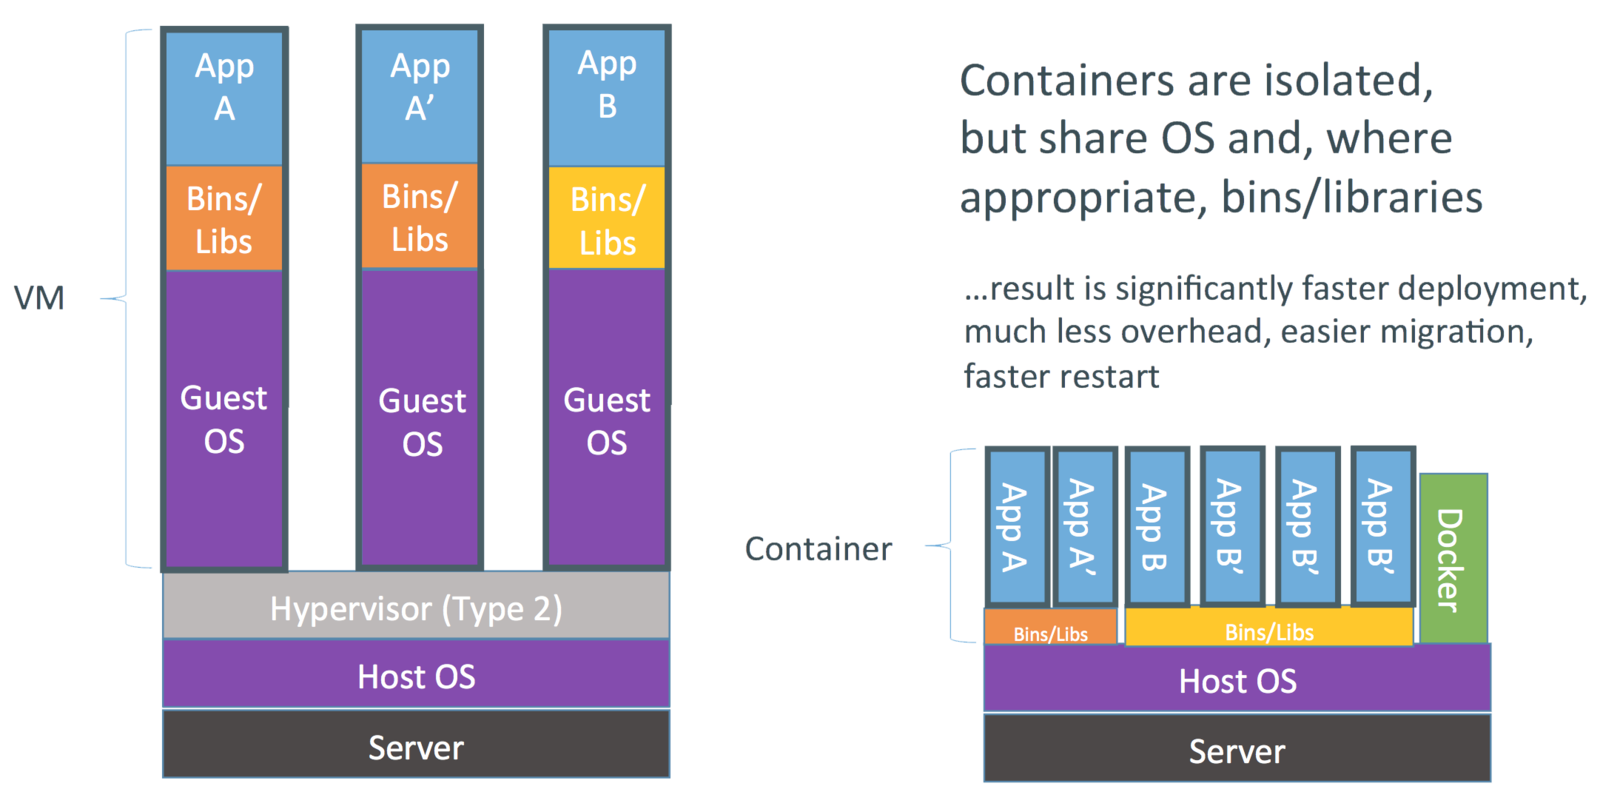
\includegraphics[width=0.8\textwidth]{media/vm-vs-cont}
  \end{center}

  \vfill

  \footnotesize{\textcolor{gray}{\url{https://dzone.com/articles/evolution-of-linux-containers-future}}}
\end{frame}

\begin{frame}{Способы работы с контейнерами}
\textbf{Существует несколько технологий контейнеризации:}

\begin{itemize}
\item \textbf{Docker} — самая популярная платформа контейнеризации
\item \textbf{Podman} — альтернатива Docker без демона
\item \textbf{LXC/LXD} — системные контейнеры
\end{itemize}

\end{frame}

\begin{frame}{Docker}
  \begin{center}
    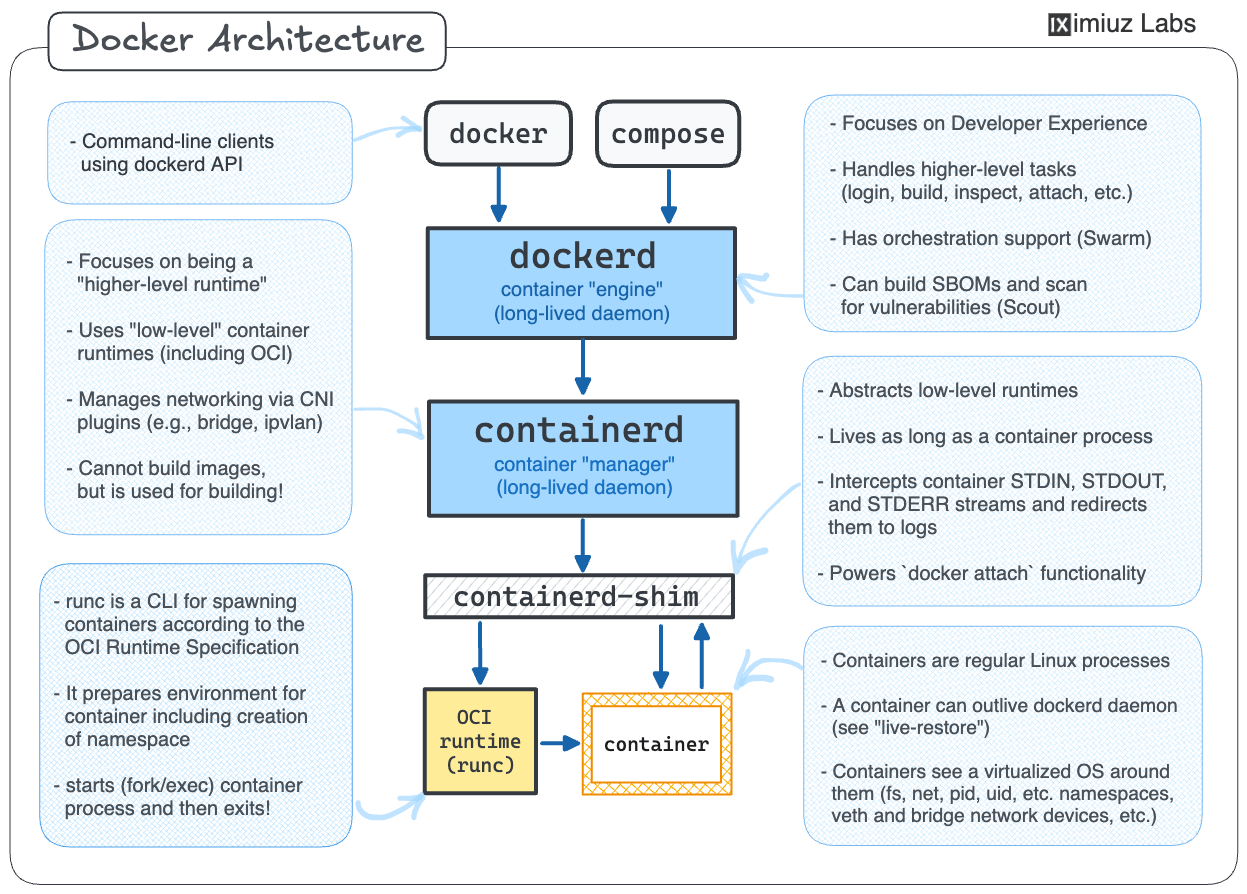
\includegraphics[width=0.64\textwidth]{media/docker-arch}
  \end{center}

  \footnotesize{\textcolor{gray}{\url{https://labs.iximiuz.com/challenges/docker-install-on-ubuntu}}}
\end{frame}

\begin{frame}{Основные понятия Docker}
\textbf{Ключевые абстракции Docker:}

\begin{itemize}
  \item \textbf{Container} — процесс или группа процессов, запущенные в изолированном окружении
  \item \textbf{Image} — шаблон контейнера, содержащий снимок файловой системы и метаданные
  \item \textbf{Dockerfile} — инструкции для сборки образа (image)
\end{itemize}

\vspace{0.3cm}

\textbf{Принцип работы:}
\begin{enumerate}
\item Описываем как собрать образ в Dockerfile
\item Собираем образ из Dockerfile
\item Запускаем контейнер из образа
\end{enumerate}
\end{frame}


\begin{frame}{Docker контейнер}
  \begin{center}
    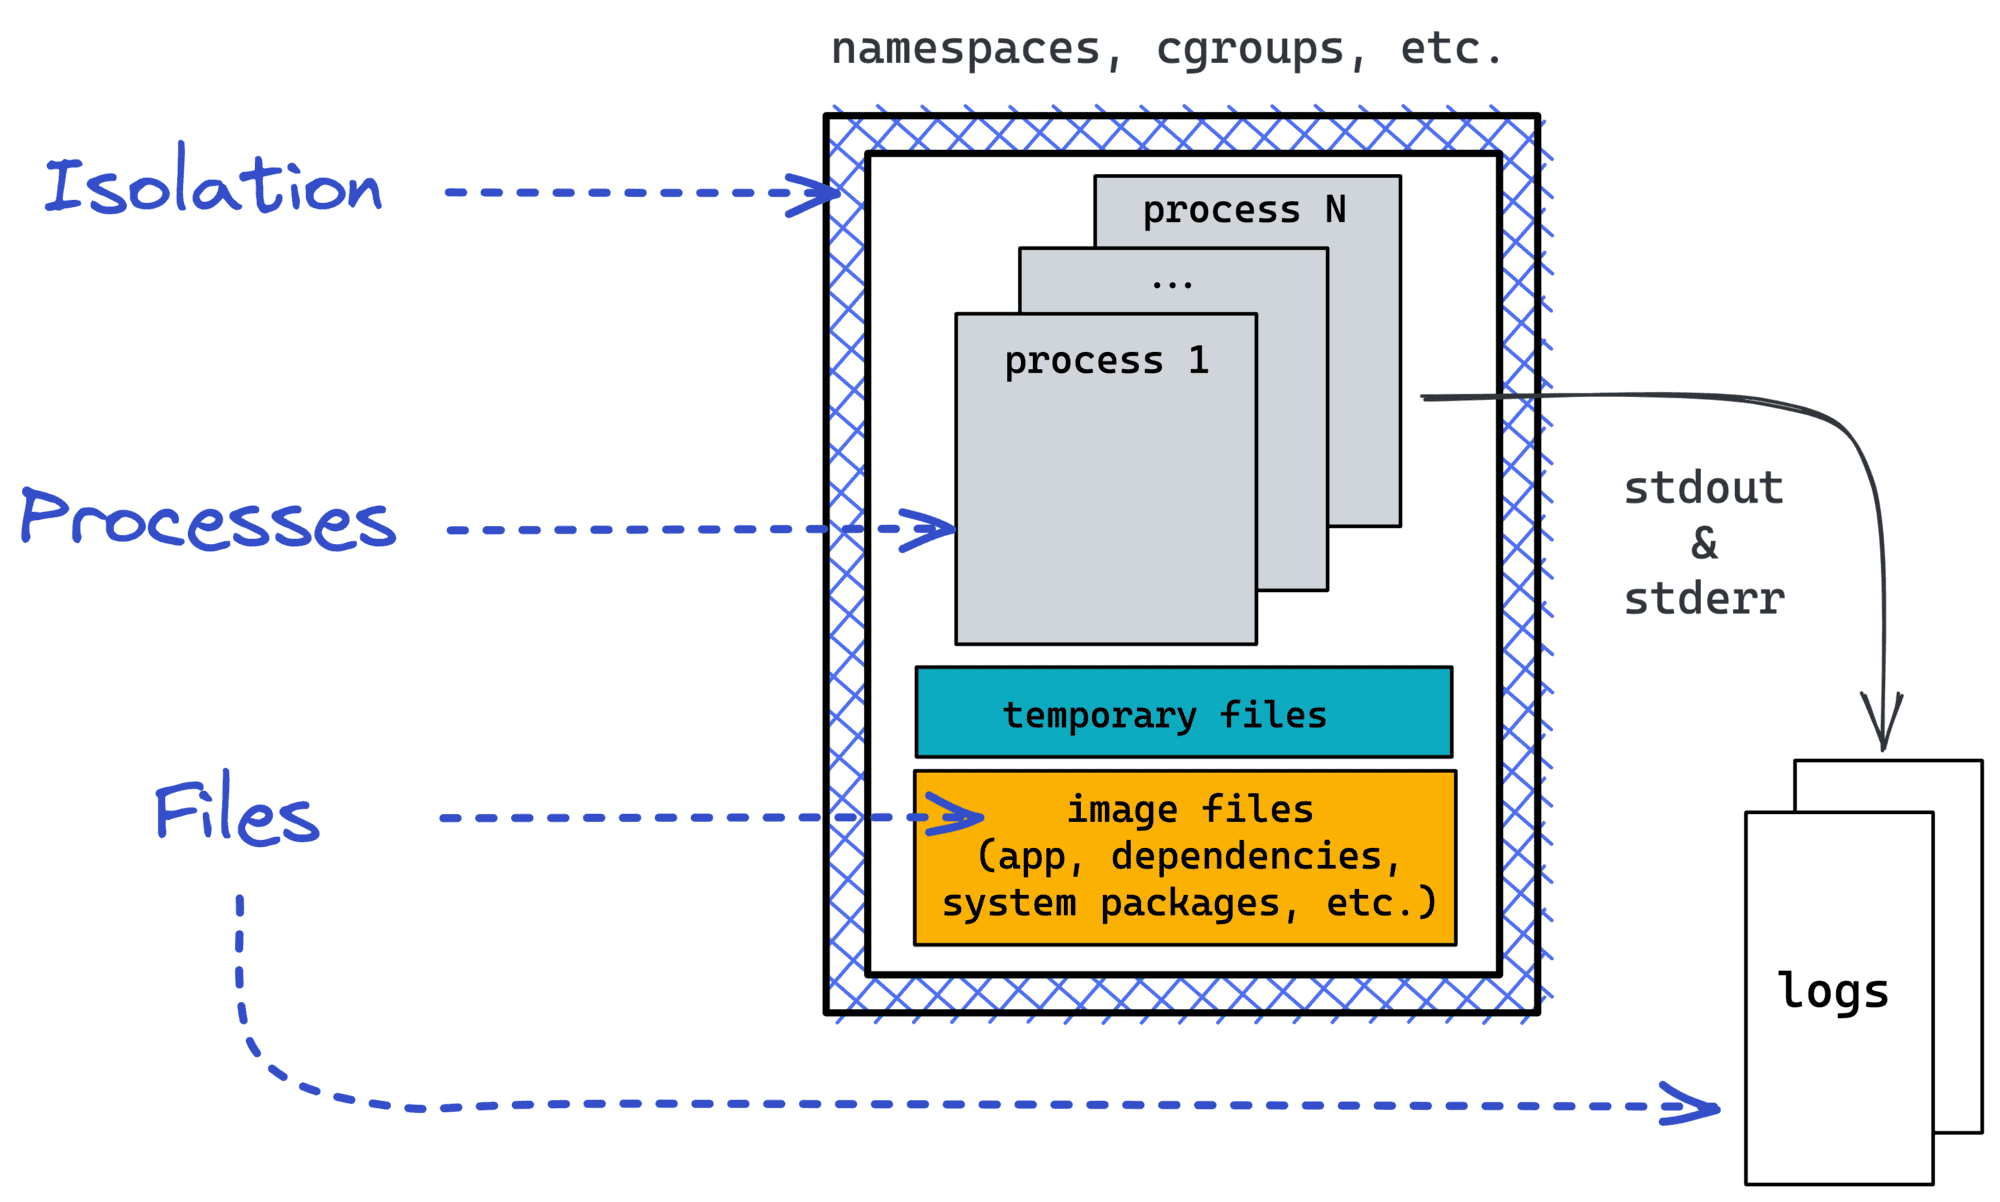
\includegraphics[width=0.8\textwidth]{media/container-is}
  \end{center}

  \footnotesize{\textcolor{gray}{\url{https://labs.iximiuz.com/tutorials/docker-container-management-commands}}}

\end{frame}

\begin{frame}{Docker Registry}

\textbf{Docker Registry} — это сервер для хранения и распространения Docker-образов.

Примеры:
\begin{itemize}
  \item Docker Hub
  \item GitLab Registry
  \item GitHub Container Registry
  \item Harbor
\end{itemize}

\vspace{0.5cm}

\textbf{Основные операции:}
\begin{itemize}
\item \textbf{Push} — загрузка образа в удаленный registry
\item \textbf{Pull} — скачивание образа из registry
\end{itemize}
\end{frame}

\begin{frame}{Docker Image}
  \begin{center}
    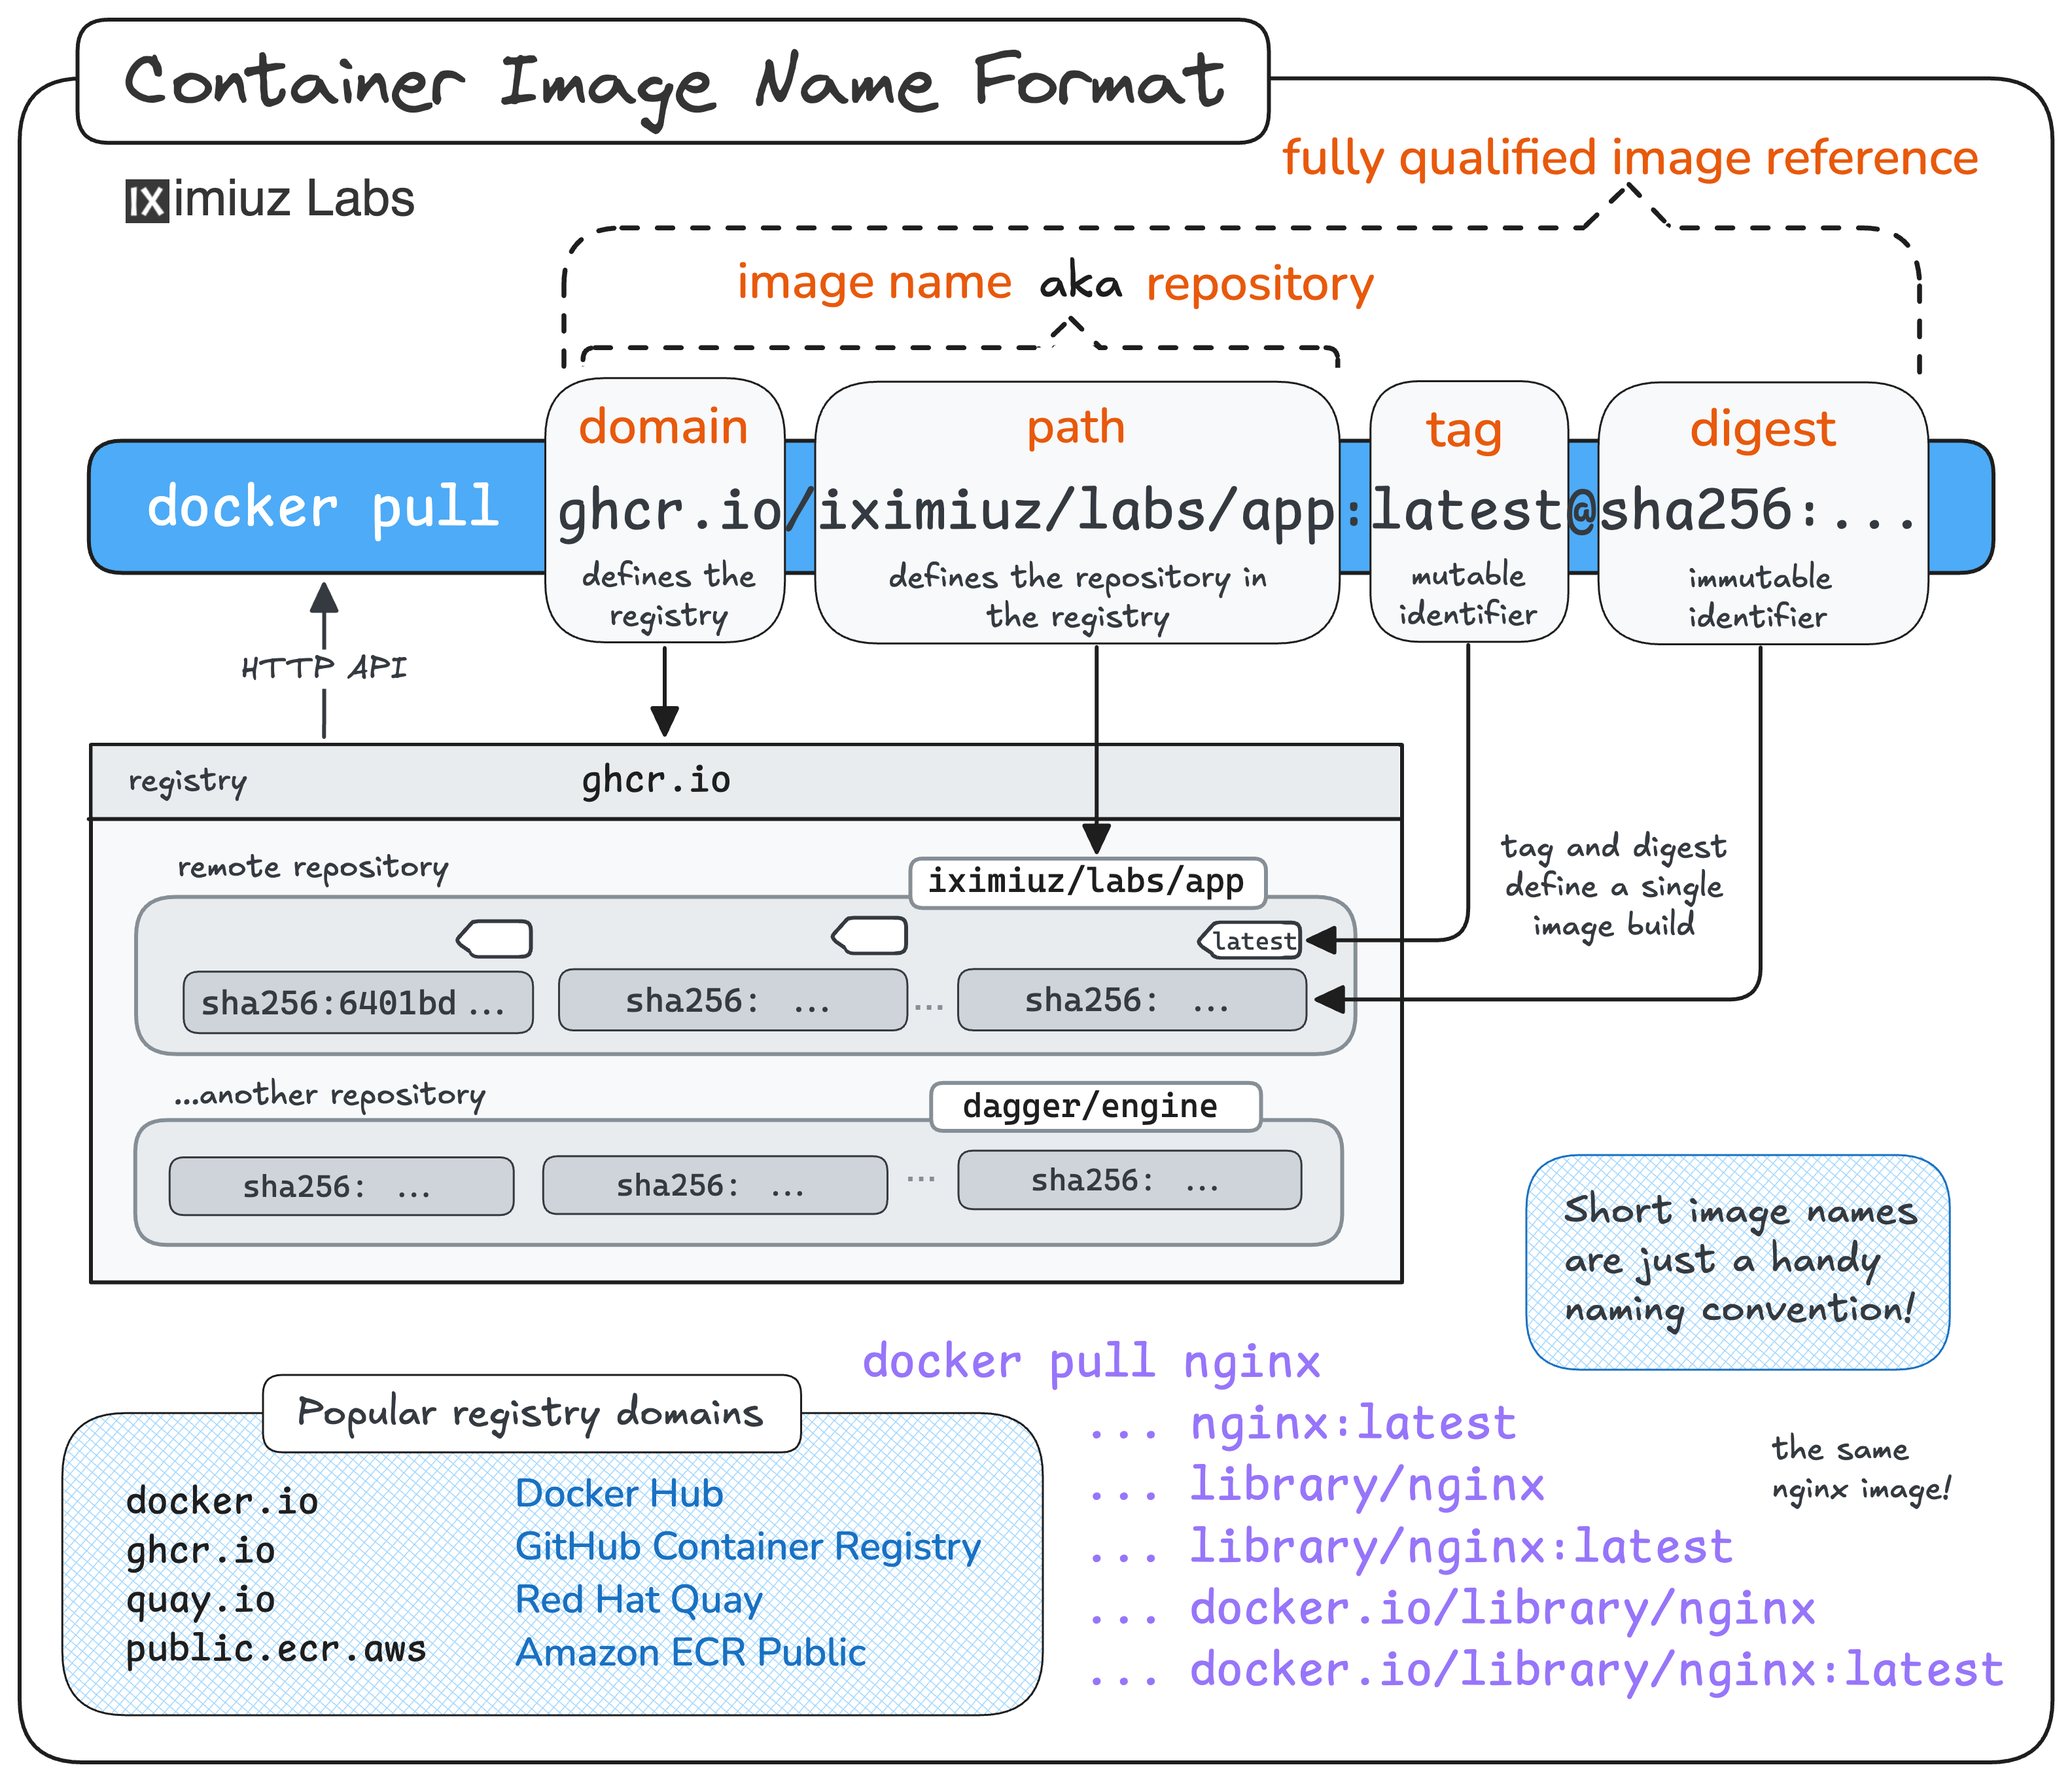
\includegraphics[width=0.5\textwidth]{media/image-format}
  \end{center}

  \footnotesize{\textcolor{gray}{\url{https://labs.iximiuz.com/challenges/build-and-publish-container-image-with-docker}}}

\end{frame}

\begin{frame}{Демонстрация: Docker Image, Container, Registry}
  \textbf{Что покажем:}
  \begin{enumerate}
    \item Устройство слоёв имеджей
    \item Базовая работа с контейнерами через docker cli
    \item Работа с docker registry
  \end{enumerate}

  \vspace{0.2cm}

  \textbf{Демо-репозиторий:} \\
  \href{https://github.com/prafdin/devops-course-demos/tree/docker}{\texttt{https://github.com/prafdin/devops-course-demos/tree/docker}}

\end{frame}

\begin{frame}{Демонстрация: Контейнеризация сайта}
\textbf{Что покажем:}
\begin{enumerate}
\item Dockerfile для сайта
\item Работа с контейнерами через docker cli
\item Использование контейнера в CI/CD пайплайне
\end{enumerate}

\vspace{0.2cm}

\textbf{Демо-репозиторий:} \\
\href{https://github.com/prafdin/devops-demo-website/tree/docker-demo}{\texttt{https://github.com/prafdin/devops-demo-website/tree/docker-demo}}

\end{frame}

\section{Docker в CI/CD}

\begin{frame}{Эволюция нашего pipeline}
\begin{columns}[t]
\begin{column}[t]{0.5\textwidth}
\textbf{Было:}
\begin{itemize}
\item Ansible устанавливаете nginx
\item deploy.sh копирует файлы
\end{itemize}
\end{column}

\begin{column}[t]{0.5\textwidth}
\textbf{Стало:}
\begin{itemize}
\item Ansible устанавливает только docker
\item Docker build, push в pipeline
\item Запуск на сервере
\end{itemize}
\end{column}
\end{columns}
\end{frame}



\section{Заключение}

\begin{frame}{Что запомнить}
\begin{itemize}
\item \textbf{Контейнеризация} — ключевой принцип современной инфраструктуры
\item \textbf{Контейнеризация решает проблемы} переносимости и конфликтов зависимостей
\item \textbf{Контейнеризация стандартизирует окружение} и упрощает развертывание
\end{itemize}

\vspace{1cm}
\begin{center}
\textbf{Вопросы?}
\end{center}
\end{frame}

\end{document}